\documentclass[12pt]{article} % Set base font size to 12pt
\usepackage{graphicx}
\usepackage{geometry} % Adjust page margins
\usepackage{setspace} % Line spacing
\usepackage{titlesec} % Customize section titles
\usepackage{tocloft} % Customize table of contents
\usepackage{fancyhdr} % Headers and footers
\usepackage{hyperref} % Add hyperlinks
\usepackage{xcolor} % Color package
\usepackage[T1]{fontenc} % Proper font encoding
\usepackage[utf8]{inputenc} % UTF-8 encoding
\usepackage[ngerman]{babel} % German language support

% Set page margins
\geometry{a4paper, margin=2.5cm}

% Set line spacing
\setstretch{1.5} % Adjust line spacing for better readability

% Customize section titles
\titleformat{\section}[block]{\LARGE\bfseries\color{black}}{}{0em}{\filcenter}
\titlespacing*{\section}{0pt}{3.5ex plus 1ex minus .2ex}{2.3ex plus .2ex}

% Customize table of contents
\renewcommand{\cftsecleader}{\cftdotfill{\cftdotsep}}
\renewcommand{\contentsname}{Inhaltsverzeichnis}
\renewcommand{\cftaftertoctitle}{\par\nobreak\bigskip\bigskip\bigskip} % Add space after TOC title
\setlength{\cftbeforesecskip}{0.5em} % Adjust spacing between section entries
\setlength{\cftaftertoctitleskip}{2cm} % Adjust spacing between TOC title and entries
\hypersetup{
    colorlinks=true,
    linkcolor=blue,
    filecolor=magenta,
    urlcolor=cyan,
}

% Define headers and footers
\pagestyle{fancy}
\fancyhf{} % Clear default headers and footers
\fancyhead[R]{\thepage} % Page number on right side of header
\fancyhead[L]{\nouppercase{\leftmark}} % Chapter title on left side of header
\renewcommand{\headrulewidth}{0pt} % Remove header line
\fancyfoot[C]{\thepage} % Page number in the center of footer
\renewcommand{\footrulewidth}{0pt} % Remove footer line

% Define light gray color
\definecolor{lightgray}{RGB}{240,240,240}

\begin{document}

% Title Page
\begin{titlepage}
    \centering
    \vspace*{3cm}
    {\Huge\bfseries\textcolor{blue}{\MakeUppercase{ Studentleben }}\par} % Increased font size and colored title
    \vspace{0.5cm} % Adjust space between title and author
    {\Large\textit{ Maja Schmidt }\par} % Italic author name
    \vfill
    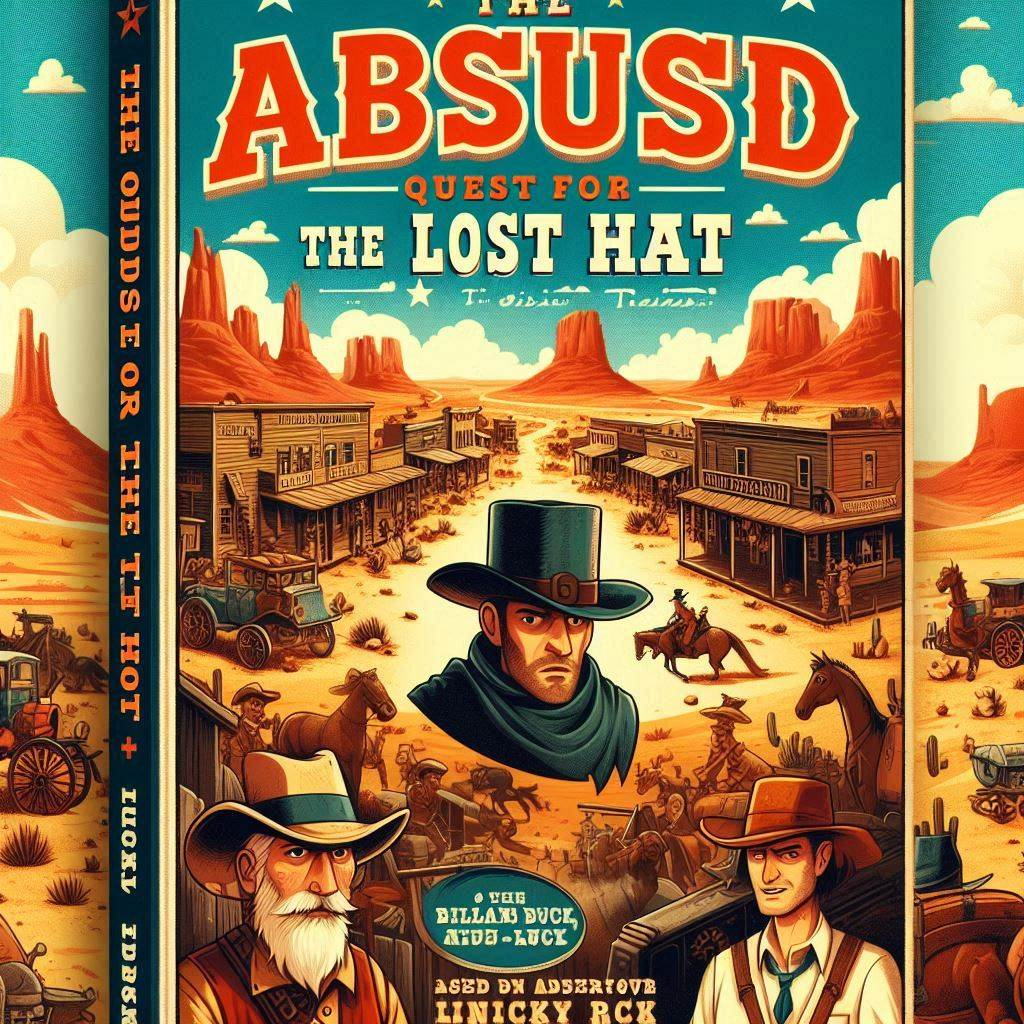
\includegraphics[width=0.9\textwidth]{ cover.jpg } % Larger cover image
    \vfill
    \today
\end{titlepage}

% Autorenvita
\section*{Autorenvita}
\vspace{4cm} % Adjust space between "Autorenvita" and "Inhaltsverzeichnis"
Maja Schmidt ist eine erfahrene Autorin, die sich auf romantische Geschichten über das Studentenleben spezialisiert hat. Mit ihrem einfühlsamen Schreibstil und ihrer Fähigkeit, realistische Erfahrungen mit romantischen Elementen zu verweben, hat sie bereits eine treue Leserschaft gewonnen. Ihre Bücher bieten eine fesselnde und inspirierende Leseerfahrung, die junge Erwachsene anspricht und in die Welt des Studentenlebens eintauchen lässt.

% Place table of contents on a separate page
\clearpage
\tableofcontents
\clearpage

% Chapters

\section{ Neue Anfänge }
 Sophie war aufgeregt, als sie den ersten Schritt auf den Universitätscampus setzte. Alles war so neu und aufregend. Sie spürte eine Mischung aus Nervosität und Vorfreude, als sie sich umsah und die vielen Gebäude und Gesichter auf sich wirken ließ. Inmitten des Trubels erkannte sie plötzlich eine vertraute Gestalt. Es war Lena, ihre beste Freundin seit Kindertagen. Die beiden umarmten sich stürmisch und begannen sofort, die neuen Möglichkeiten des Studentenlebens zu erkunden. Gemeinsam besuchten sie die Orientierungsveranstaltungen und lernten die verschiedenen Clubs und Aktivitäten auf dem Campus kennen. Es fühlte sich gut an, eine vertraute Person an ihrer Seite zu haben, während sie sich in dieser neuen Umgebung zurechtfinden musste. Doch trotz Lenas Unterstützung fühlte sich Sophie auch ein wenig unsicher. Sie fragte sich, ob sie den Anforderungen des Studiums gewachsen sein würde und ob sie neue Freunde finden könnte. Diese Gedanken begleiteten sie, als sie sich auf den Weg zu ihrer ersten Vorlesung machte. Dort begegnete sie Max zum ersten Mal. Er saß in der ersten Reihe, lächelte sie an und bot ihr einen Platz neben sich an. Sophie spürte sofort eine gewisse Anziehungskraft zwischen ihnen und war neugierig darauf, mehr über ihn zu erfahren. Während der Vorlesung entdeckten sie, dass sie einige Gemeinsamkeiten hatten, und verabredeten sich, um sich nach der Vorlesung auf einen Kaffee zu treffen. Diese Begegnung sollte der Beginn einer besonderen Verbindung sein, die Sophie und Max auf eine Reise voller Herausforderungen und Erfolge im Studentenleben führen würde. Sophie und Max verbrachten den Nachmittag damit, sich näher kennenzulernen. Sie teilten ihre Träume, Ängste und Hoffnungen miteinander und fanden heraus, dass sie viele gemeinsame Interessen hatten. Während ihres Gesprächs entdeckten sie, dass sie beide eine Leidenschaft für das Reisen und die Fotografie teilten. Max erzählte von seinen Abenteuern in fernen Ländern, und Sophie berichtete von ihrer Begeisterung für die faszinierende Architektur und Kultur verschiedener Städte. Es war, als ob sie sich schon lange kennen würden, und doch war da auch eine aufregende Spannung, die sie beide spürten. Als die Sonne langsam unterging, beschlossen sie, gemeinsam zum Abendessen zu gehen. Auf dem Weg zum Restaurant tauschten sie Geschichten aus ihrer Vergangenheit aus und lachten über lustige Erlebnisse. Es fühlte sich an, als ob sie sich in einer Blase befanden, in der nur sie beide existierten. Doch die Realität holte sie ein, als sie das Restaurant betraten und auf Lena trafen, die bereits auf sie wartete. Lena strahlte vor Freude, als sie die beiden sah, und schien zu ahnen, dass sich zwischen Sophie und Max etwas Besonderes entwickelte. Während des Abendessens erzählte Lena von ihren eigenen Abenteuern und Herausforderungen, und die drei Freunde verbrachten einen unvergesslichen Abend miteinander. Als sie sich später voneinander verabschiedeten, wussten Sophie und Max, dass sich ihr Leben für immer verändert hatte, und sie freuten sich auf die gemeinsamen Herausforderungen, die noch vor ihnen lagen. Sophie fühlte sich dankbar für Lenas Unterstützung, als sie sich in der neuen Umgebung zurechtfinden musste. Die anfängliche Unsicherheit wich langsam einem Gefühl der Aufregung und Abenteuerlust. Max war stets an ihrer Seite, ermutigte sie, sich neuen Herausforderungen zu stellen, und half ihr, ihre Leidenschaft für Architektur und Kultur weiter zu entfalten. Gemeinsam erkundeten sie die Campusstadt und entdeckten versteckte Ecken, die sie mit ihrer Kamera festhielten. In diesen Momenten fühlte sich Sophie lebendiger und freier als je zuvor. Professor Müller ermutigte sie, ihre kreativen Interessen zu verfolgen und eröffnete ihr neue Perspektiven. Die Freundschaft zwischen Sophie, Max und Lena wuchs mit jeder gemeinsamen Erfahrung. Als sie sich später voneinander verabschiedeten, wussten sie, dass sich ihr Leben für immer verändert hatte, und sie freuten sich auf die gemeinsamen Herausforderungen, die noch vor ihnen lagen.

\section{ Liebe im Uni-Alltag }
 Sophie und Max verbrachten immer mehr Zeit miteinander, vertieften ihre Beziehung und entdeckten, dass sie sich ineinander verliebt hatten. Die gemeinsamen Höhen und Tiefen des Uni-Alltags schweißten sie noch enger zusammen. Während Sophie sich mit den Anforderungen des Studiums auseinandersetzte, fand sie in Lena eine unterstützende Freundin, die sie ermutigte, weiterzumachen. Max hingegen suchte Rat bei Professor Müller, der ihm wichtige Ratschläge gab, wie er seine Leidenschaft für Architektur und Design mit seinem Studium verbinden konnte. Die Unterstützung von Freunden und Mentoren half beiden, ihre eigenen Wege zu finden und sich in der neuen Umgebung zurechtzufinden. Inmitten des Uni-Alltags erlebten Sophie und Max ein unerwartetes Ereignis, das sie noch näher zusammenbrachte. Sie lernten, dass Liebe und Unterstützung in schwierigen Zeiten besonders wichtig sind und dass sie gemeinsam jede Herausforderung meistern konnten. Als Sophie und Max sich tiefer in ihre Beziehung vertieften, wurden sie mit neuen Herausforderungen konfrontiert, die ihr Band auf die Probe stellten. Der Uni-Alltag brachte nicht nur gemeinsame Höhen, sondern auch Tiefen mit sich, die sie gemeinsam meistern mussten. Während Sophie sich weiterhin mit den Anforderungen des Studiums auseinandersetzte, fand sie in Lena eine unterstützende Freundin, die sie ermutigte, weiterzumachen. Lena selbst musste ihre eigenen Herausforderungen meistern, was ihre Freundschaft mit Sophie auf eine neue Ebene brachte. Max hingegen suchte weiterhin Rat bei Professor Müller, der ihm half, seine Leidenschaft für Architektur und Design mit seinem Studium zu verbinden. Die Gespräche mit Professor Müller eröffneten Max neue Perspektiven und halfen ihm, seine Ziele klarer zu definieren. Die Unterstützung von Freunden und Mentoren erwies sich als entscheidend, als Sophie und Max mit unerwarteten Schwierigkeiten konfrontiert wurden. Inmitten des Uni-Alltags und der damit verbundenen Herausforderungen lernten sie, dass Liebe und Unterstützung in schwierigen Zeiten besonders wichtig sind. Ihr gemeinsames Band wurde durch das Überwinden von Hindernissen gestärkt, und sie erkannten, dass sie gemeinsam jede Herausforderung meistern konnten, solange sie füreinander da waren. Als der Semesterstress zunahm, fanden sich Sophie und Max inmitten von Prüfungsvorbereitungen und Projektarbeiten wieder. Die Anforderungen des Studiums forderten ihren Tribut, und sie mussten lernen, wie sie ihre Zeit effektiv nutzen konnten, um den Herausforderungen gerecht zu werden. In dieser stressigen Zeit fanden sie Trost und Unterstützung in ihrer Beziehung, die ihnen die nötige Kraft gab, um durchzuhalten. Sophie war entschlossen, sich den Prüfungen zu stellen, aber Zweifel nagten dennoch an ihr. Max erkannte ihre Unsicherheit und stand ihr bei, indem er sie ermutigte und an ihre Fähigkeiten glaubte. 'Du bist so talentiert, Sophie. Du schaffst das', sagte er sanft, während er ihre Hand hielt. Diese Worte gaben Sophie die Zuversicht, die sie brauchte, um sich ihren Ängsten zu stellen. Währenddessen fand Lena in ihrer eigenen Prüfungsphase Unterstützung bei Professor Müller, der ihr half, ihre Leidenschaft für Geschichte mit ihren akademischen Verpflichtungen in Einklang zu bringen. 'Sie haben das Potenzial, die Welt der Geschichte zu verändern', ermutigte er sie. Diese Worte beflügelten Lena und gaben ihr die Motivation, die sie brauchte, um sich den Herausforderungen zu stellen. Inmitten des Prüfungsstresses fanden Sophie, Max und Lena Trost und Ermutigung in ihrer Freundschaft und den weisen Ratschlägen ihres Mentors. Sie erkannten, dass sie gemeinsam stark waren und dass ihre Liebe und Unterstützung füreinander unersetzlich waren, besonders in Zeiten der Prüfungen und Unsicherheiten.

\section{ Herausforderungen und Überwindungen }
 Die Sonne strahlte über dem Campus, als Emma und Lukas sich in der Bibliothek trafen, um gemeinsam an einem wichtigen Projekt zu arbeiten. Die bevorstehenden Prüfungen und die Anforderungen des Studiums hatten sie beide in Beschlag genommen, und dennoch fanden sie Trost und Motivation in ihrer gemeinsamen Entschlossenheit, ihre Ziele zu erreichen. Während Emma sich auf ihre akademischen Ziele konzentrierte, spürte sie die Unterstützung und den Rückhalt von Lukas, der sie mit seiner ruhigen Entschlossenheit inspirierte. Inmitten von Büchern und Notizen fanden sie einen gemeinsamen Rhythmus, der ihre Zusammenarbeit effektiv und harmonisch gestaltete. Gleichzeitig standen Sarah und David vor familiären Herausforderungen, die ihre Aufmerksamkeit und Energie erforderten. Trotz der Belastungen fanden sie Wege, einander beizustehen und sich gegenseitig zu stärken. Die Freundschaften vertieften sich, während die Charaktere lernten, dass sie gemeinsam jede Herausforderung überwinden konnten. Die Universität und die Stadt Sonnenstadt wurden zum Zeugen ihrer Entschlossenheit und ihres Zusammenhalts, während sie sich den Herausforderungen des Studiums und des Lebens mutig stellten. Die Sonne neigte sich langsam über den Campus, als Emma und Lukas sich in ihrem Lieblingscafé trafen, um eine dringend benötigte Pause von ihren Studien zu machen. Die letzten Wochen hatten sie vor große Herausforderungen gestellt, und nun war es an der Zeit, sich zu entspannen und neue Energie zu tanken. Während sie ihre heißen Getränke schlürften, tauschten sie Geschichten über ihre Kindheit aus und lachten über lustige Erlebnisse aus ihrer Vergangenheit. Es war ein Moment der Leichtigkeit und Freude, der sie daran erinnerte, dass das Leben mehr war als nur Prüfungen und Verpflichtungen. Gleichzeitig führte Sarah ein tiefgründiges Gespräch mit David über ihre Zukunft und ihre Träume. Sie ermutigten sich gegenseitig, ihre Ziele zu verfolgen und sich nicht von Hindernissen entmutigen zu lassen. Die Worte, die sie austauschten, waren wie ein Anker in stürmischen Zeiten, der ihnen Halt und Zuversicht gab. Als die Sterne am Abendhimmel erschienen, spürten die Charaktere, dass sie gestärkt und bereit waren, sich den kommenden Herausforderungen zu stellen. Ihre Freundschaften und Beziehungen hatten in diesen Momenten der Überwindung eine neue Tiefe und Bedeutung gewonnen, und sie wussten, dass sie gemeinsam alles erreichen konnten, was das Leben für sie bereithielt. Die Sonne neigte sich langsam über den Campus, als Emma und Lukas sich in ihrem Lieblingscafé trafen, um eine dringend benötigte Pause von ihren Studien zu machen. Die letzten Wochen hatten sie vor große Herausforderungen gestellt, und nun war es an der Zeit, sich zu entspannen und neue Energie zu tanken. Während sie ihre heißen Getränke schlürften, tauschten sie Geschichten über ihre Kindheit aus und lachten über lustige Erlebnisse aus ihrer Vergangenheit. Es war ein Moment der Leichtigkeit und Freude, der sie daran erinnerte, dass das Leben mehr war als nur Prüfungen und Verpflichtungen. Gleichzeitig führte Sarah ein tiefgründiges Gespräch mit David über ihre Zukunft und ihre Träume. Sie ermutigten sich gegenseitig, ihre Ziele zu verfolgen und sich nicht von Hindernissen entmutigen zu lassen. Die Worte, die sie austauschten, waren wie ein Anker in stürmischen Zeiten, der ihnen Halt und Zuversicht gab. Als die Sterne am Abendhimmel erschienen, spürten die Charaktere, dass sie gestärkt und bereit waren, sich den kommenden Herausforderungen zu stellen. Ihre Freundschaften und Beziehungen hatten in diesen Momenten der Überwindung eine neue Tiefe und Bedeutung gewonnen, und sie wussten, dass sie gemeinsam alles erreichen konnten, was das Leben für sie bereithielt.

\section{ Erfolge und Feiern }
 Die Sonne strahlte golden über dem Campus, als Emma und Lukas sich auf dem grünen Rasen versammelten, um ihre Erfolge im Studium zu feiern. Die frische Brise trug die fröhlichen Klänge der Musikwettbewerbe und die jubelnden Rufe der Studenten, die sich in verschiedenen Aktivitäten engagierten. Emma strahlte vor Stolz, als sie Lukas in die Arme fiel und ihm für seine unermüdliche Unterstützung dankte. 'Ohne dich hätte ich das niemals geschafft', flüsterte sie ihm zu, und er lächelte und erwiderte: 'Wir haben es gemeinsam geschafft, und ich bin so stolz auf dich.' Sarah und David gesellten sich zu ihnen, und sie stießen mit prickelndem Sekt auf ihre Erfolge an. 'Auf die Zukunft und auf die unzähligen Abenteuer, die noch vor uns liegen', rief Sarah und hob ihr Glas. Die Charaktere lachten, tanzten und genossen den Moment des Triumphs, der ihre harte Arbeit und ihre unerschütterliche Freundschaft feierte. Inmitten des fröhlichen Trubels fanden sie einen ruhigen Moment, um über ihre persönlichen Wachstum und die Bedeutung von Freundschaft und Liebe zu reflektieren. 'Es war nicht immer einfach, aber es war jede Anstrengung wert', sagte David und lächelte Sarah an. Die Sonne neigte sich langsam dem Horizont zu, und die Charaktere wussten, dass sie bereit waren, die nächsten Schritte zu gehen, gestärkt durch ihre Erfolge und die tiefe Verbundenheit, die sie miteinander teilten. Die Nacht brach langsam über Sonnenstadt herein, als Emma und Lukas Hand in Hand am Ufer des malerischen Sees spazierten. Das sanfte Plätschern des Wassers und der klare Sternenhimmel bildeten eine romantische Kulisse für ihre Gedanken und Gefühle. 'Es fühlt sich an, als ob alles möglich ist, wenn du an meiner Seite bist', sagte Emma leise und lächelte verträumt. Lukas zog sie sanft an sich und erwiderte: 'Du bist mein größter Erfolg, Emma. Mit dir an meiner Seite fühle ich mich unbesiegbar.' In diesem Moment der Intimität und Verbundenheit erkannten sie, dass ihre Liebe stark genug war, um jede Herausforderung zu meistern. Zur gleichen Zeit fanden Sarah und David in einem gemütlichen Café Zuflucht vor der Hektik des Alltags. Bei Kerzenschein und leiser Musik tauschten sie Blicke voller Vertrauen und Zuneigung aus. 'Unsere Erfolge sind auch die Erfolge unserer Liebe und Freundschaft', sagte Sarah und griff nach Davids Hand. 'Gemeinsam können wir alles erreichen', antwortete David und lächelte liebevoll. Die Charaktere erkannten, dass ihre Erfolge nicht nur individuell, sondern auch gemeinsam gefeiert werden sollten. Sie wussten, dass ihre Freundschaft und Liebe die Grundlage für all ihre zukünftigen Abenteuer bildeten, und sie waren bereit, sich den kommenden Herausforderungen mit vereinten Kräften zu stellen. Die Nacht brach langsam über Sonnenstadt herein, als Emma und Lukas Hand in Hand am Ufer des malerischen Sees spazierten. Das sanfte Plätschern des Wassers und der klare Sternenhimmel bildeten eine romantische Kulisse für ihre Gedanken und Gefühle. 'Es fühlt sich an, als ob alles möglich ist, wenn du an meiner Seite bist', sagte Emma leise und lächelte verträumt. Lukas zog sie sanft an sich und erwiderte: 'Du bist mein größter Erfolg, Emma. Mit dir an meiner Seite fühle ich mich unbesiegbar.' In diesem Moment der Intimität und Verbundenheit erkannten sie, dass ihre Liebe stark genug war, um jede Herausforderung zu meistern. Zur gleichen Zeit fanden Sarah und David in einem gemütlichen Café Zuflucht vor der Hektik des Alltags. Bei Kerzenschein und leiser Musik tauschten sie Blicke voller Vertrauen und Zuneigung aus. 'Unsere Erfolge sind auch die Erfolge unserer Liebe und Freundschaft', sagte Sarah und griff nach Davids Hand. 'Gemeinsam können wir alles erreichen', antwortete David und lächelte liebevoll. Die Charaktere erkannten, dass ihre Erfolge nicht nur individuell, sondern auch gemeinsam gefeiert werden sollten. Sie wussten, dass ihre Freundschaft und Liebe die Grundlage für all ihre zukünftigen Abenteuer bildeten, und sie waren bereit, sich den kommenden Herausforderungen mit vereinten Kräften zu stellen. Die Nacht verstrich, aber die Erinnerungen an diesen Abend der Verbundenheit und Feierlichkeit würden für immer in ihren Herzen bleiben.

\section{ Abschied und Neuanfang }
 Die Abschlussfeier näherte sich mit großen Schritten, und die Atmosphäre an der Universität war von Aufregung und Wehmut erfüllt. Emma und Lukas standen am Ufer des malerischen Sees, wo sie so viele unvergessliche Momente miteinander geteilt hatten. Ein Hauch von Melancholie lag in der Luft, als sie sich in die Augen sahen und die Unsicherheit der Zukunft spürten. 'Es wird seltsam sein, nicht mehr jeden Tag hier zu sein', gestand Emma mit einem Anflug von Wehmut. Lukas umarmte sie sanft und sagte: 'Aber wir haben so viele wundervolle Erinnerungen, die uns für immer verbinden werden. Egal, wohin das Leben uns führt, wir werden immer einen Teil von Sonnenstadt in unseren Herzen tragen.' Die Worte beruhigten Emma und gaben ihr die Gewissheit, dass ihre Zeit an der Universität zwar enden mochte, ihre Verbindung zu Lukas jedoch für immer bestehen würde. Währenddessen saßen Sarah und David auf einer Bank im idyllischen Universitätsgarten und ließen ihre Gedanken über die vergangenen Jahre schweifen. 'Es fühlt sich an, als ob wir gerade erst angefangen haben, und jetzt ist es schon vorbei', seufzte Sarah. David nahm ihre Hand und antwortete: 'Aber wir haben so viel gemeinsam erlebt und erreicht. Unsere Freundschaft und Liebe haben uns durch Höhen und Tiefen getragen, und das wird auch in Zukunft so sein.' Die beiden spürten die Wehmut des Abschieds, aber auch die Vorfreude auf die neuen Wege, die vor ihnen lagen. Die Charaktere standen am Beginn eines neuen Kapitels in ihrem Leben, bereit, sich den Herausforderungen und Chancen zu stellen, die die Zukunft für sie bereithielt. Die Abschlussfeier näherte sich mit großen Schritten, und die Atmosphäre an der Universität war von Aufregung und Wehmut erfüllt. Emma und Lukas standen am Ufer des malerischen Sees, wo sie so viele unvergessliche Momente miteinander geteilt hatten. Ein Hauch von Melancholie lag in der Luft, als sie sich in die Augen sahen und die Unsicherheit der Zukunft spürten. 'Es wird seltsam sein, nicht mehr jeden Tag hier zu sein', gestand Emma mit einem Anflug von Wehmut. Lukas umarmte sie sanft und sagte: 'Aber wir haben so viele wundervolle Erinnerungen, die uns für immer verbinden werden. Egal, wohin das Leben uns führt, wir werden immer einen Teil von Sonnenstadt in unseren Herzen tragen.' Die Worte beruhigten Emma und gaben ihr die Gewissheit, dass ihre Zeit an der Universität zwar enden mochte, ihre Verbindung zu Lukas jedoch für immer bestehen würde. Währenddessen saßen Sarah und David auf einer Bank im idyllischen Universitätsgarten und ließen ihre Gedanken über die vergangenen Jahre schweifen. 'Es fühlt sich an, als ob wir gerade erst angefangen haben, und jetzt ist es schon vorbei', seufzte Sarah. David nahm ihre Hand und antwortete: 'Aber wir haben so viel gemeinsam erlebt und erreicht. Unsere Freundschaft und Liebe haben uns durch Höhen und Tiefen getragen, und das wird auch in Zukunft so sein.' Die beiden spürten die Wehmut des Abschieds, aber auch die Vorfreude auf die neuen Wege, die vor ihnen lagen. Die Charaktere standen am Beginn eines neuen Kapitels in ihrem Leben, bereit, sich den Herausforderungen und Chancen zu stellen, die die Zukunft für sie bereithielt. Als die Sonne langsam unterging, umarmten sich die vier Freunde und schworen sich, dass ihre Freundschaft und Liebe für immer bestehen würde, egal wohin das Leben sie führen würde. Die Abschlussfeier war ein emotionaler Höhepunkt, der die Charaktere mit Stolz und Wehmut erfüllte. Emma stand auf der Bühne, um ihre Abschlussrede zu halten, und ließ ihren Blick über die versammelten Studenten schweifen. 'Wir haben gemeinsam gelacht, geweint, gekämpft und gesiegt. Jeder von uns hat seine eigenen Herausforderungen gemeistert und ist daran gewachsen', begann sie mit leidenschaftlicher Stimme. 'Aber das Wichtigste ist, dass wir uns gegenseitig unterstützt und ermutigt haben. Unsere Freundschaften haben uns stark gemacht, und sie werden uns auch in Zukunft begleiten.' Die Menge applaudierte begeistert, und Emma spürte, wie sich die Bande der Gemeinschaft um sie herum verstärkten. Währenddessen stand Lukas inmitten seiner Kommilitonen, stolz auf das, was sie gemeinsam erreicht hatten. Er umarmte Emma voller Stolz, und seine Augen strahlten vor Liebe und Bewunderung. 'Du hast sie alle inspiriert und berührt', flüsterte er ihr zu. 'Du bist ein wahrer Stern, der die Welt erhellt.' Emma lächelte gerührt und wusste, dass Lukas immer an ihrer Seite sein würde, egal wohin das Leben sie führen mochte. Sarah und David genossen den festlichen Abend, umgeben von Freunden und geliebten Menschen. Sie tanzten gemeinsam und ließen die Musik und die Freude des Augenblicks auf sich wirken. 'Es fühlt sich an, als ob wir fliegen könnten', lachte Sarah, während David sie voller Anmut über das Parkett führte. 'Ja, weil wir gemeinsam alles schaffen können', antwortete David mit einem strahlenden Lächeln. Die Charaktere spürten die tiefe Verbundenheit und das Vertrauen, das sie füreinander empfanden. Die Abschlussfeier markierte nicht nur das Ende ihres Studiums, sondern auch den Beginn eines neuen Kapitels, in dem ihre Freundschaften und Beziehungen weiter erblühen würden.

\clearpage

% Metadata
\section*{Metadaten}
\colorbox{lightgray}{
    \begin{minipage}{\dimexpr\textwidth-2\fboxsep}
        \vspace{1cm}
        \begin{itemize}
            \item Name des Buches: Studentleben
            \item Name des Autors: Maja Schmidt
            \item Name des Herausgebers: Mark Zimmermann
            \item Name des Verlags: HdM AI Technologies
            \item Adresse des Verlags: Nobelstraße 10, 70569 Stuttgart
            \item Datum der Veröffentlichung: 2022-10-20
        \end{itemize}
        \vspace{1cm}
    \end{minipage}
}

\end{document}